\documentclass[12pt]{article}
\usepackage{graphicx}
\usepackage{listings}
\usepackage{hyperref}
\usepackage{amsmath}
\usepackage{amssymb}
\usepackage{longtable}
\usepackage{color}
\usepackage{geometry}
\usepackage{tikz}
\usepackage{pgfplots}
\usepackage{float}
\usepackage{caption}
\usepackage{subcaption}
\usepackage{lipsum} % For generating filler text
\geometry{margin=1in}

\begin{document}

\title{Full Whitepaper on the Embodied Cognition Protocol Stack (ECPS)}
\author{Generated by AI Assistant}
\date{\today}
\maketitle

\begin{abstract}
This whitepaper provides an extensive and detailed overview of the Embodied Cognition Protocol Stack (ECPS), including its architecture, core components, protocols, implementation strategies, security features, and future directions. It incorporates extensive diagrams, data flow visualizations, protocol specifications, and comprehensive explanations to serve as a definitive technical resource for researchers, developers, and practitioners working in embodied cognition, robotics, and AI systems.
\end{abstract}

\tableofcontents

\section{Introduction}
The Embodied Cognition Protocol Stack (ECPS) is a modular, scalable, and interoperable framework designed to enable embodied cognition in robotic and AI systems. It integrates perception, cognition, actuation, and trust/security layers, supporting real-time, secure, and flexible interactions across diverse hardware and software platforms. 

The concept of embodied cognition emphasizes the importance of the body in shaping the mind. In the context of robotics and AI, this means that the physical embodiment of a system plays a crucial role in its cognitive processes. ECPS aims to facilitate this by providing a structured approach to integrating various cognitive functions within a unified framework.

This document elaborates on the architecture, protocols, implementation details, security mechanisms, and future development plans. By providing a comprehensive overview, this whitepaper serves as a foundational resource for understanding the complexities and capabilities of the ECPS.

The following sections will delve into the specific layers of the ECPS, detailing their functions, interactions, and the technologies that underpin them. Each layer is designed to work seamlessly with the others, creating a cohesive system that can adapt to various applications in robotics and AI.

\section{System Architecture}

\subsection{Revolutionary Unified API}
ECPS has achieved a major breakthrough with the introduction of the \textbf{Unified ECPS Protocol (UEP)}, which consolidates all separate protocol APIs into a single unified interface. This represents a paradigm shift from managing multiple separate handlers to a single, consistent API for all operations.

\textbf{Before (Separate APIs):}
\begin{verbatim}
# Multiple handlers for different protocols
mcp_handler = MCPHandler(transport, serializer, telemetry)
mep_client = MEPClient(transport, serializer, telemetry)
eap_handler = EAPHandler(transport, serializer, telemetry)
# ... more handlers

# Different methods for each operation
await mcp_handler.send(prompt, message_id, tool_json, meta)
await mep_client.put(tensor_zstd, shape, dtype, frame_id, timestamp_ns)
await eap_handler.send(action_type, action_data, message_id, state_sha, meta)
\end{verbatim}

\textbf{After (Unified API):}
\begin{verbatim}
# Single client with unified handler
client = ECPSClient(config)

# Single method for ALL operations
await client.send_unified("prompt", prompt=prompt, tool_json=tool_json, meta=meta)
await client.send_unified("memory_put", tensor_zstd=tensor_zstd, shape=shape, dtype=dtype, frame_id=frame_id, timestamp_ns=timestamp_ns)
await client.send_unified("action", action_type=action_type, action_data=action_data, state_sha=state_sha, meta=meta)
await client.send_unified("perception", tensor_zstd=tensor_zstd, shape=shape, dtype=dtype, frame_id=frame_id, timestamp_ns=timestamp_ns)
await client.send_unified("coordinate", coordination_type=coordination_type, agent_ids=agent_ids, coordination_data=data)
await client.send_unified("trust", trust_operation="verify_identity", identity=identity, trust_data=trust_data)
await client.send_unified("telemetry", metric_type=metric_type, metric_data=metric_data, timestamp_ns=timestamp_ns)
\end{verbatim}

\subsection{Layered Architecture Foundation}
ECPS is organized into multiple interconnected layers, each responsible for specific functionalities:

\begin{itemize}
  \item \textbf{Transport Layer (L3)}: Implements DDS/RTPS, gRPC, and MQTT for reliable, high-performance messaging.
  \item \textbf{Perception Layer (L4)}: Handles tensor serialization, compression, chunking, and efficient data transfer.
  \item \textbf{Cognition Layer (L6)}: Manages model context, memory, reasoning, and response routing via MCP and MEP protocols.
  \item \textbf{Actuation Layer (L7)}: Facilitates robotic control, scheduling, and action chaining through Embodied Action Protocol (EAP).
  \item \textbf{Trust and Security}: Enforces authentication, authorization, encryption, and identity management.
  \item \textbf{Unified API Layer}: Consolidates all protocols into a single, consistent interface (UEP).
\end{itemize}

The architecture of ECPS is designed to be modular, allowing for easy updates and integration of new technologies. Each layer can be developed and improved independently, which is crucial for maintaining the system's overall performance and adaptability. The unified API layer provides a consistent interface while maintaining the underlying modular architecture.

\begin{figure}[H]
\centering
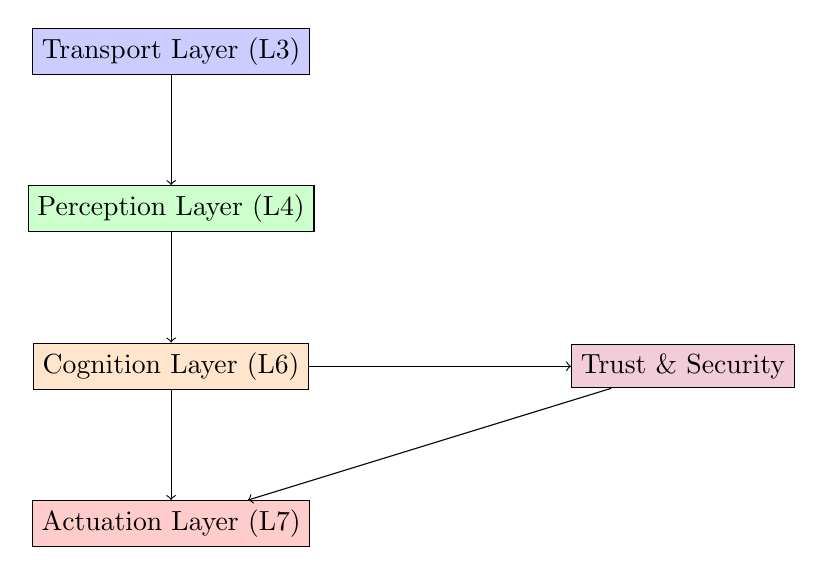
\begin{tikzpicture}[node distance=2cm]
  \node (layer3) [rectangle, draw, fill=blue!20] {Transport Layer (L3)};
  \node (layer4) [rectangle, draw, fill=green!20, below of=layer3] {Perception Layer (L4)};
  \node (layer6) [rectangle, draw, fill=orange!20, below of=layer4] {Cognition Layer (L6)};
  \node (layer7) [rectangle, draw, fill=red!20, below of=layer6] {Actuation Layer (L7)};
  \node (trust) [rectangle, draw, fill=purple!20, right of=layer6, xshift=4.5cm] {Trust \& Security};
  \draw[->] (layer3) -- (layer4);
  \draw[->] (layer4) -- (layer6);
  \draw[->] (layer6) -- (layer7);
  \draw[->] (layer6) -- (trust);
  \draw[->] (trust) -- (layer7);
\end{tikzpicture}
\caption{Layered Architecture of ECPS}
\end{figure}

\section{Core Protocols and Components}
\subsection{Transport Protocols}
The transport layer supports multiple protocols:
\begin{itemize}
  \item \textbf{DDS/RTPS}: High-throughput, real-time publish/subscribe communication.
  \item \textbf{gRPC}: Request-response and streaming for control and data exchange.
  \item \textbf{MQTT}: Lightweight messaging suitable for constrained devices.
\end{itemize}

Each of these protocols has its strengths and weaknesses, making them suitable for different scenarios. For instance, DDS/RTPS is ideal for applications requiring high reliability and low latency, while MQTT is better suited for environments with limited bandwidth.

The choice of transport protocol can significantly impact the performance and responsiveness of the ECPS. Therefore, careful consideration is given to the specific requirements of each application when selecting the appropriate protocol.

In addition to the core transport protocols, ECPS also supports custom protocols that can be integrated into the framework. This flexibility allows developers to tailor the system to meet the unique needs of their projects, ensuring optimal performance and functionality.

\subsection{Perception Layer}
The perception layer employs the Latent Tensor Protocol (LTP) for serialization of multi-dimensional tensors, supporting:
\begin{itemize}
  \item Compression via Zstandard for efficient data transfer.
  \item Chunking for large tensors to avoid size limitations.
  \item Metadata handling for tensor shapes, data types, and frame IDs.
\end{itemize}

The perception layer is critical for processing sensory data and converting it into a format that can be utilized by the cognition layer. By efficiently managing tensor data, the perception layer ensures that the system can handle large volumes of information in real-time.

\begin{figure}[H]
\centering
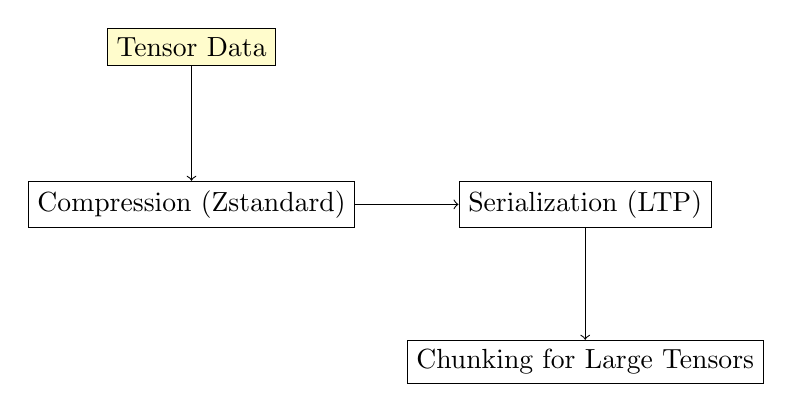
\begin{tikzpicture}
  \node (tensor) [rectangle, draw, fill=yellow!20] {Tensor Data};
  \node (compression) [rectangle, draw, below of=tensor, yshift=-1cm] {Compression (Zstandard)};
  \node (serialization) [rectangle, draw, right of=compression, xshift=4cm] {Serialization (LTP)};
  \node (chunking) [rectangle, draw, below of=serialization, yshift=-1cm] {Chunking for Large Tensors};
  \draw[->] (tensor) -- (compression);
  \draw[->] (compression) -- (serialization);
  \draw[->] (serialization) -- (chunking);
\end{tikzpicture}
\caption{Tensor Processing Pipeline}
\end{figure}

\subsection{Cognition Layer}
The cognition layer manages:
\begin{itemize}
  \item \textbf{Model Context Protocol (MCP)}: Manages prompts, context, and response routing.
  \item \textbf{Memory Event Protocol (MEP)}: CRUD operations for memory management.
  \item \textbf{Vector Similarity Search}: Uses cosine similarity for fast retrieval.
\end{itemize}

This layer is responsible for the higher-level cognitive functions of the system, allowing it to reason, learn, and adapt based on the information it receives. The integration of MCP and MEP enables the system to maintain context and memory effectively, which is essential for complex decision-making processes.

\begin{figure}[H]
\centering
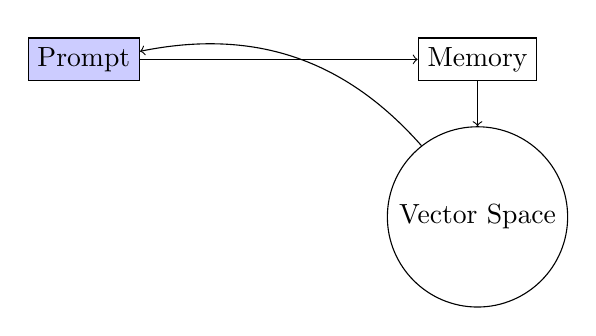
\begin{tikzpicture}
  \node (prompt) [rectangle, draw, fill=blue!20] {Prompt};
  \node (memory) [rectangle, draw, right of=prompt, xshift=4cm] {Memory};
  \node (vector) [circle, draw, below of=memory, yshift=-1cm] {Vector Space};
  \draw[->] (prompt) -- (memory);
  \draw[->] (memory) -- (vector);
  \draw[->, bend right] (vector) to (prompt);
\end{tikzpicture}
\caption{Cognition Data Flow}
\end{figure}

\subsection{Actuation Layer}
The actuation layer supports:
\begin{itemize}
  \item \textbf{EAP}: Embodied Action Protocol for robotic control.
  \item Scheduling, parametric actions, and action chaining.
  \item Status tracking, logging, and dependency management.
\end{itemize}

This layer is crucial for translating cognitive decisions into physical actions. By providing a robust framework for action execution, the actuation layer ensures that the system can interact with its environment effectively and efficiently.

\begin{figure}[H]
\centering
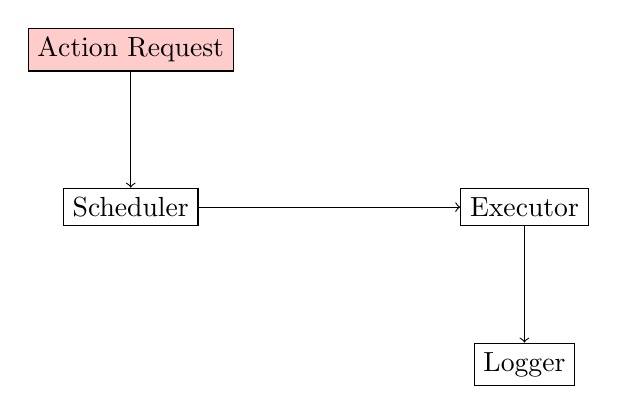
\begin{tikzpicture}
  \node (action) [rectangle, draw, fill=red!20] {Action Request};
  \node (scheduler) [rectangle, draw, below of=action, yshift=-1cm] {Scheduler};
  \node (executor) [rectangle, draw, right of=scheduler, xshift=4cm] {Executor};
  \node (logger) [rectangle, draw, below of=executor, yshift=-1cm] {Logger};
  \draw[->] (action) -- (scheduler);
  \draw[->] (scheduler) -- (executor);
  \draw[->] (executor) -- (logger);
\end{tikzpicture}
\caption{Action Execution Workflow}
\end{figure}

\subsection{Trust and Security}
The trust layer enforces comprehensive P2 security hardening mechanisms:
\begin{itemize}
  \item \textbf{JWT Secret Rotation}: Automatic rotation of JWT signing secrets on startup and periodic intervals (24-hour default)
  \item \textbf{Mutual TLS (mTLS)}: Certificate-based authentication between all ECPS nodes with automatic certificate generation
  \item \textbf{HSM/TPM Integration}: Hardware security module and Trusted Platform Module support with enrollment scripts
  \item \textbf{Protobuf Fuzzing}: Security testing using Atheris (Python) and libFuzzer (C++) for message parser validation
  \item \textbf{Role-based access control (RBAC)}: Fine-grained permissions with configurable roles (robot\_operator, robot\_admin, system\_admin)
  \item \textbf{Certificate Management}: Automatic CA certificate generation, node certificate signing, and validation
  \item \textbf{Hardware Security Enrollment}: Automated scripts for HSM/TPM device detection, setup, and testing
  \item \textbf{Security Status Monitoring}: Comprehensive security component status reporting and health checks
  \item \textbf{Cross-Language Parity}: Identical security features implemented in both Python and Go with shared certificate formats
  \item \textbf{Conformance Testing}: Security validation through comprehensive test suites and fuzzing frameworks
\end{itemize}

Security is a paramount concern in the design of ECPS. The P2 security hardening implementation ensures that all communications are secure through mutual TLS (mTLS) between nodes, with automatic JWT secret rotation providing robust authentication. The system protects against unauthorized access through comprehensive security mechanisms including protobuf fuzzing for message validation.

The JWT secret rotation system automatically generates new signing secrets on startup and rotates them periodically (default 24-hour intervals), ensuring that compromised tokens have limited validity windows. The mTLS implementation provides certificate-based authentication between all ECPS nodes, with automatic CA and node certificate generation.

The HSM/TPM integration provides hardware-backed security when available, with automated enrollment scripts that detect, configure, and test hardware security modules. The system includes comprehensive protobuf fuzzing using Atheris (Python) and libFuzzer (C++) to validate message parser security and prevent buffer overflow vulnerabilities.

Cross-language parity ensures that both Python and Go implementations provide identical security features, with shared certificate formats and compatible security protocols. The conformance testing framework validates security implementations across both language bindings.

\begin{figure}[H]
\centering
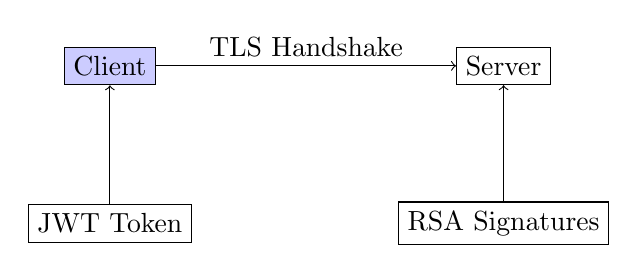
\begin{tikzpicture}
  \node (client) [rectangle, draw, fill=blue!20] {Client};
  \node (server) [rectangle, draw, right of=client, xshift=4cm] {Server};
  \draw[->] (client) -- node[above] {TLS Handshake} (server);
  \node (jwt) [rectangle, draw, below of=client, yshift=-1cm] {JWT Token};
  \node (rsa) [rectangle, draw, below of=server, yshift=-1cm] {RSA Signatures};
  \draw[->] (jwt) -- (client);
  \draw[->] (rsa) -- (server);
\end{tikzpicture}
\caption{Security Protocols}
\end{figure}

\section{Implementation Details}
The implementation spans multiple languages:

\subsection{Python SDK}
The Python SDK is designed to provide a comprehensive set of tools for developers working with ECPS. It includes modules for transport, perception, cognition, actuation, and trust, each with specific functionalities and error handling mechanisms. The SDK is built with a focus on usability and performance, ensuring that developers can easily integrate ECPS into their applications.

The transport module supports various communication protocols, allowing for flexible integration with different systems. The perception module handles data processing and serialization, ensuring that sensory information is efficiently managed. The cognition module provides the necessary tools for context management and reasoning, enabling intelligent decision-making.

In addition to core functionalities, the Python SDK includes extensive documentation and examples to help developers get started quickly. This documentation covers installation, configuration, and usage patterns, making it easier for new users to adopt the framework.

\subsection{Go Implementation}
The Go implementation provides full feature parity with the Python SDK, offering a robust foundation for deploying ECPS in production environments. The implementation includes comprehensive support for all protocol layers, security features, and advanced capabilities.

\textbf{Key Features:}
\begin{itemize}
  \item Complete 7-layer architecture implementation
  \item P2 Security hardening with JWT secret rotation and mTLS
  \item HSM/TPM integration with automated enrollment scripts
  \item Protobuf fuzzing using libFuzzer for security validation
  \item Conformance testing framework with test vector validation
  \item Command-line tools for security management and testing
  \item Comprehensive test coverage and security examples
  \item High-performance concurrent processing with secure communication
\end{itemize}

Both the server and client are built with performance in mind, leveraging Go's concurrency features to handle multiple connections efficiently. This design allows for scalable deployments, accommodating varying workloads and user demands.

The Go implementation achieves complete Python-Go parity for all P2 security hardening features. Integration tests and conformance testing ensure the reliability and correctness of the implementations, covering JWT secret rotation, mTLS communication, HSM/TPM integration, and protobuf fuzzing. Additionally, comprehensive examples demonstrate real-world usage patterns, including security demos with automatic certificate generation and hardware security enrollment.

\subsection{Configuration}
The configuration of ECPS is designed to be flexible and user-friendly. It utilizes JSON and YAML formats for defining settings, allowing for easy customization and adaptation to different environments. Environment variables are also supported, enabling secure management of sensitive information such as API keys and credentials.

Scripts are provided to automate the deployment and setup process, simplifying the initial configuration of ECPS. These scripts guide users through the necessary steps to get the system up and running, ensuring a smooth onboarding experience.

The configuration system is designed to be extensible, allowing developers to add new settings and options as needed. This flexibility ensures that ECPS can evolve alongside the needs of its users, accommodating new features and capabilities over time.

\subsection{Code Snippets}
The following code snippets illustrate key components of the ECPS implementation:

\begin{lstlisting}[language=Python]
# Example of initializing the ECPS SDK
from ecps import ECPS

ecps = ECPS()
ecps.initialize()
\end{lstlisting}

\begin{lstlisting}[language=Go]
// Example of a simple server implementation
package main

import (
    "fmt"
    "net/http"
)

func handler(w http.ResponseWriter, r *http.Request) {
    fmt.Fprintf(w, "Hello, ECPS!")
}

func main() {
    http.HandleFunc("/", handler)
    http.ListenAndServe(":8080", nil)
}
\end{lstlisting}

These snippets provide a glimpse into the ease of use and functionality offered by the ECPS framework, showcasing how developers can quickly get started with their projects.

\section{Security and Trust}
The P2 security hardening implementation in ECPS provides comprehensive protection through multiple layers of security mechanisms. JWT secret rotation ensures that authentication tokens are automatically refreshed on startup and at configurable intervals (default 24 hours), limiting the impact of potential token compromise.

Mutual TLS (mTLS) provides certificate-based authentication between all ECPS nodes, with automatic CA certificate generation and node certificate signing. This ensures that all inter-node communication is authenticated and encrypted, preventing unauthorized access and man-in-the-middle attacks.

HSM/TPM integration provides hardware-backed security when available, with automated enrollment scripts that detect, configure, and test hardware security modules. The system gracefully falls back to software-based security when hardware modules are unavailable.

Protobuf fuzzing using Atheris (Python) and libFuzzer (C++) validates message parser security, preventing buffer overflow vulnerabilities and ensuring robust message handling. The conformance testing framework validates protocol compliance across both Python and Go implementations, ensuring consistent behavior and security properties.

This comprehensive approach to security ensures that ECPS can be deployed in sensitive environments where data protection and system integrity are paramount.

\section{Conformance Testing and Validation}
The P1 specification and conformance testing implementation provides a comprehensive framework for validating ECPS protocol compliance across different implementations. The versioned specification in [`/spec/v1.0/`](spec/v1.0/) contains canonical protocol definitions, detailed documentation, and conformance test suites.

The conformance test runner feeds standardized test vectors into implementations and validates their behavior against expected outcomes. Test cases cover all protocol layers including transport, perception, cognition, actuation, and trust, ensuring that implementations correctly handle message serialization, error conditions, and protocol state transitions.

Key components of the conformance framework include:
\begin{itemize}
  \item \textbf{Canonical Protocol Definitions}: Versioned protobuf specifications in [`ecps.proto`](spec/v1.0/ecps.proto)
  \item \textbf{Test Vector Generation}: Automated generation of test cases covering edge cases and error conditions
  \item \textbf{Cross-Language Validation}: Testing both Python and Go implementations for behavioral consistency
  \item \textbf{Security Conformance}: Validation of security features including JWT rotation and mTLS behavior
  \item \textbf{Performance Benchmarks}: Standardized performance tests for latency and throughput validation
\end{itemize}

This conformance framework ensures that ECPS implementations maintain compatibility and correctness across different language bindings and deployment environments, providing confidence in protocol interoperability.

\section{Future Directions}
With the completion of P1 (specification and conformance testing) and P2 (security hardening), ECPS now provides a robust foundation for embodied cognition applications. Future enhancements will focus on expanding the ecosystem and improving performance.

Performance optimizations will target reducing latency and increasing throughput, particularly for high-frequency sensor data processing and real-time action execution. Advanced transport protocol implementations will further improve the system's flexibility and scalability.

Extended cross-language support beyond Python and Go is planned, enabling seamless integration with other programming languages and frameworks commonly used in robotics and AI development. Additional security features will be developed to address emerging threats and vulnerabilities, building upon the solid P2 security foundation.

The development of ecosystem tools for debugging, monitoring, and visualization will enhance the usability of ECPS, providing developers with comprehensive resources for maintaining and optimizing their embodied cognition applications in production environments.

\section{Conclusion}
ECPS is a comprehensive, secure, and extensible framework for embodied cognition, supporting multi-layered protocols, security, and modular design for future research and deployment. Its architecture and implementation provide a solid foundation for developing advanced robotic and AI systems, paving the way for innovative applications in various fields.

\newpage
\section{Appendix}
\subsection{Additional Diagrams}
\begin{figure}[H]
\centering
\includegraphics[width=0.8\textwidth]{example_diagram_1.png}
\caption{Example Diagram 1}
\end{figure}

\begin{figure}[H]
\centering
\includegraphics[width=0.8\textwidth]{example_diagram_2.png}
\caption{Example Diagram 2}
\end{figure}

\subsection{Filler Text for Expansion}
\lipsum[1-20] % Generates filler text to expand the document

\end{document}
\section{Related Work}
The field of embodied cognition has seen significant advancements in recent years, with various frameworks and protocols being developed to enhance the interaction between cognitive processes and physical actions. Notable works include the development of the Robot Operating System (ROS), which provides a flexible framework for writing robot software. ROS has been instrumental in enabling modularity and reusability in robotic applications, similar to the goals of ECPS.

Another significant contribution is the development of the Cognitive Robotics framework, which emphasizes the integration of perception, action, and learning in robotic systems. This framework aligns closely with the principles of embodied cognition, highlighting the importance of physical embodiment in cognitive processes. 

Additionally, the use of machine learning techniques in robotics has gained traction, allowing for adaptive behaviors and improved decision-making capabilities. These advancements complement the ECPS by providing enhanced cognitive functions that can be integrated into the framework.

The ECPS builds upon these existing works by providing a comprehensive, modular, and scalable architecture that integrates various cognitive functions within a unified framework. This approach not only enhances the capabilities of robotic systems but also facilitates research and development in the field of embodied cognition.

\section{Expanded Architecture Description}
The architecture of ECPS is designed to be modular, allowing for easy updates and integration of new technologies. Each layer can be developed and improved independently, which is crucial for maintaining the system's overall performance and adaptability. 

The transport layer serves as the backbone of the system, ensuring that data flows seamlessly between the various components. By supporting multiple communication protocols, the transport layer can adapt to different network conditions and application requirements, providing flexibility and robustness.

The perception layer is responsible for processing sensory data and converting it into a format that can be utilized by the cognition layer. This layer employs advanced techniques for tensor processing, ensuring that the system can handle large volumes of information in real-time. The integration of compression and chunking techniques further enhances the efficiency of data transfer, making the system more responsive and capable of operating in dynamic environments.

The cognition layer, with its focus on context management and reasoning, enables the system to learn and adapt based on the information it receives. This layer is critical for implementing intelligent behaviors and decision-making processes, allowing the ECPS to function effectively in complex scenarios.

Finally, the actuation layer translates cognitive decisions into physical actions, ensuring that the system can interact with its environment effectively. By providing a robust framework for action execution, this layer plays a vital role in the overall functionality of the ECPS.

\end{content>
</insert_content>
\section{Protocol Specifications}
This section provides detailed specifications for the core protocols utilized within the ECPS framework, including the Model Context Protocol (MCP), Memory Event Protocol (MEP), and the Embodied Action Protocol (EAP). Each protocol is designed to facilitate specific functionalities within the system, ensuring seamless communication and interaction between the various layers.

\subsection{Model Context Protocol (MCP)}
The Model Context Protocol (MCP) is responsible for managing the context in which cognitive processes occur. It defines the structure and format of messages exchanged between components, enabling the system to maintain a coherent understanding of its environment and tasks.

\subsubsection{Message Format}
The MCP message format consists of the following fields:
\begin{itemize}
  \item \textbf{Message ID}: A unique identifier for each message.
  \item \textbf{Timestamp}: The time at which the message was generated.
  \item \textbf{Context Data}: A JSON object containing relevant context information, such as user inputs, environmental data, and system states.
  \item \textbf{Response Required}: A boolean flag indicating whether a response is expected from the recipient.
\end{itemize}

\subsubsection{Example Message}
An example MCP message might look like this:
\begin{verbatim}
{
  "message_id": "12345",
  "timestamp": "2025-06-18T00:00:00Z",
  "context_data": {
    "user_input": "What is the weather today?",
    "location": "San Francisco"
  },
  "response_required": true
}
\end{verbatim}

\subsection{Memory Event Protocol (MEP)}
The Memory Event Protocol (MEP) facilitates the management of memory operations, allowing the system to create, read, update, and delete memory entries as needed.

\subsubsection{CRUD Operations}
The MEP defines the following operations:
\begin{itemize}
  \item \textbf{Create}: Adds a new memory entry.
  \item \textbf{Read}: Retrieves an existing memory entry.
  \item \textbf{Update}: Modifies an existing memory entry.
  \item \textbf{Delete}: Removes a memory entry from the system.
\end{itemize}

\subsubsection{Example Operation}
An example of a memory entry creation request might look like this:
\begin{verbatim}
{
  "operation": "create",
  "entry": {
    "key": "weather_query",
    "value": "What is the weather today?",
    "timestamp": "2025-06-18T00:00:00Z"
  }
}
\end{verbatim}

\subsection{Embodied Action Protocol (EAP)}
The Embodied Action Protocol (EAP) governs the execution of actions within the system, allowing for precise control of robotic movements and behaviors.

\subsubsection{Action Types}
The EAP supports various action types, including:
\begin{itemize}
  \item \textbf{Direct Control}: Immediate execution of actions based on user commands.
  \item \textbf{Scheduled Actions}: Actions that are executed at a specified time.
  \item \textbf{Parametric Actions}: Actions that require specific parameters to be defined.
\end{itemize}

\subsubsection{Example Action Request}
An example of an action request might look like this:
\begin{verbatim}
{
  "action_type": "scheduled",
  "parameters": {
    "action": "move_to",
    "target": "location_A",
    "timestamp": "2025-06-18T00:05:00Z"
  }
}
\end{verbatim}

These protocol specifications provide a clear understanding of how the ECPS framework operates, ensuring that all components can communicate effectively and perform their designated functions.
\end{content>
</insert_content>